\documentclass[a4paper, 12pt, babel, spanish]{article}
\usepackage{graphicx}
\usepackage{tabularx}
\usepackage{floatflt}
\usepackage{ctable}
\usepackage{array}
\usepackage[utf8]{inputenc}
\usepackage[spanish]{babel}
\usepackage{pdflscape}

\topmargin -1.5cm        
\oddsidemargin -0.04cm   
\evensidemargin -0.04cm  
\textwidth 16.59cm
\textheight 24.94cm
\parskip 7.2pt           
\parindent 0pt		  
\setlength{\heavyrulewidth}{0.1 em}

\begin{document}

\section*{Formato del paquete}

El paquete nos quedaría del siguiente modo:

\begin{center}
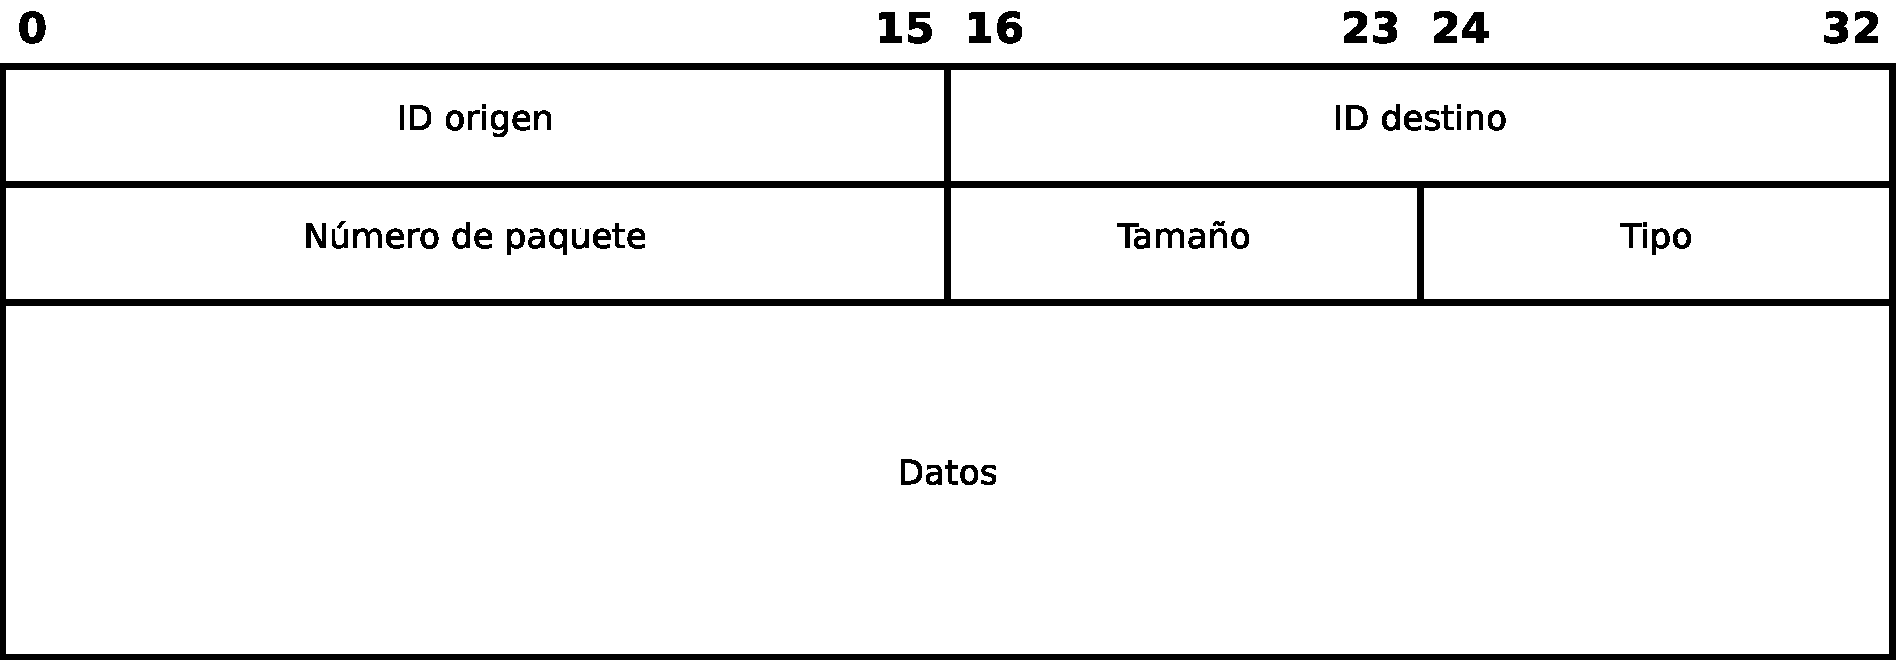
\includegraphics[width=0.7\textwidth]{fig/packet}
\end{center}

Dónde cada campo tiene la siguiente función:

\begin{itemize}
\item La ID de origen estará programada en cada NI.
\item La ID de destino será la proporcionada por el master al iniciar la transacción (con consideraciones especiales).
\item El tamaño tendrá el tamaño de los datos del paquete (en bytes).
\item El numero de paquete será un contador que llevará la NI.
\item Los tipos de paquetes los veremos a continuación en la descripción del funcionamiento de las transferencias. Actúan cómo distintos \emph{flags}, cada uno indicando la función del paquete.
\end{itemize}

\subsection*{Comentarios}

Se considerará un caso especial en el campo de la dirección de destino. Si el master inicia una ráfaga (sea del tipo que sea de las que permite el bus, la NI guardará la dirección del primer trozo a transmitirse (ya que se irá incrementando en transferencias succesivas), ya que la ID de destino se usa para el \emph{routing} y no puede ir cambiando. 

Al recibir paquetes, si se trata de una transferencia secuencial se tendrá que deshacer el cambio, sumando el tamaño de los paquetes.

\section*{Funcionamiento de las transferencias} 

\begin{floatingtable}[r]{
\begin{tabularx}{0.45\textwidth}{l X}
\toprule
\textbf{Tipo} 	& \textbf{Valor} \\ \midrule
Inicio conexión & 0000000\textbf{1} \\ \midrule
Confirmación 	& 000000\textbf{1}0 \\ \midrule
Lectura			& 00000\textbf{0}00 \\ \midrule
Escritura		& 00000\textbf{1}00 \\ \midrule
WRAP4			& 0000\textbf{1}000 \\ \midrule
WRAP8			& 000\textbf{1}0000 \\ \midrule
WRAP16			& 00\textbf{1}00000 \\
\bottomrule
\end{tabularx}}
\caption{Tipos de paquete}
\end{floatingtable}

Segun los distintos tipos de transferencia que tiene el bus \emph{AHB}, podremos tener dos grandes tipos: las operaciones de lectura y las de escritura en el bus. Por lo tanto, tendremos un tipo de paquete para cada tipo.

Al iniciar cualquier tipo de transferencia, el master pondrá en la señal \emph{HTRANS} el valor \emph{NONSEQ}. Podremos asumir que cada vez que la NI reciba esta señal se iniciará una nueva transferencia, y que si quiere enviar más datos, el master usará una ráfaga. Por lo tanto, al recibir una transferencia de este tipo, la NI pondrá a 0 el contador de paquetes y enviará un paquete de tipo \textbf{inicio de conexión}. También se guardará la dirección de destino por si lo que sigue es una ráfaga.

No se necesitará un paquete de final de conexión, ya que la NI, al recibir un paquete de inicio de conexión sabrá que se acabó la última, y del mismo modo que la interface que envía el paquete, reseteará el contador de paquetes recibidos para prepararse para la próxima transferencia.

Después de enviar cada paquete, la interface esperará la confirmación, y cuando la reciba activará la señal \emph{HREADY} para que el master siga. Según la especificación, el slave del bus debe tener un máximo de ciclos en que puede retrasar la confirmación. Se podría establecer un máximo que actuaría como timeout para hacer el reenvío del paquete (y avisar al master con la señal \emph{HRESP} poniendo el valor \emph{RETRY}.

La NI enviará un paquete de tipo \textbf{confirmación} cuando reciba un paquete de datos.

Para que pueda recibir datos, tanto la NI cómo el procesador seran master y slave. Así, cuando la interfaz reciba algun paquete podrá pedir el bus y enviarle la información al procesador: 

\begin{center}
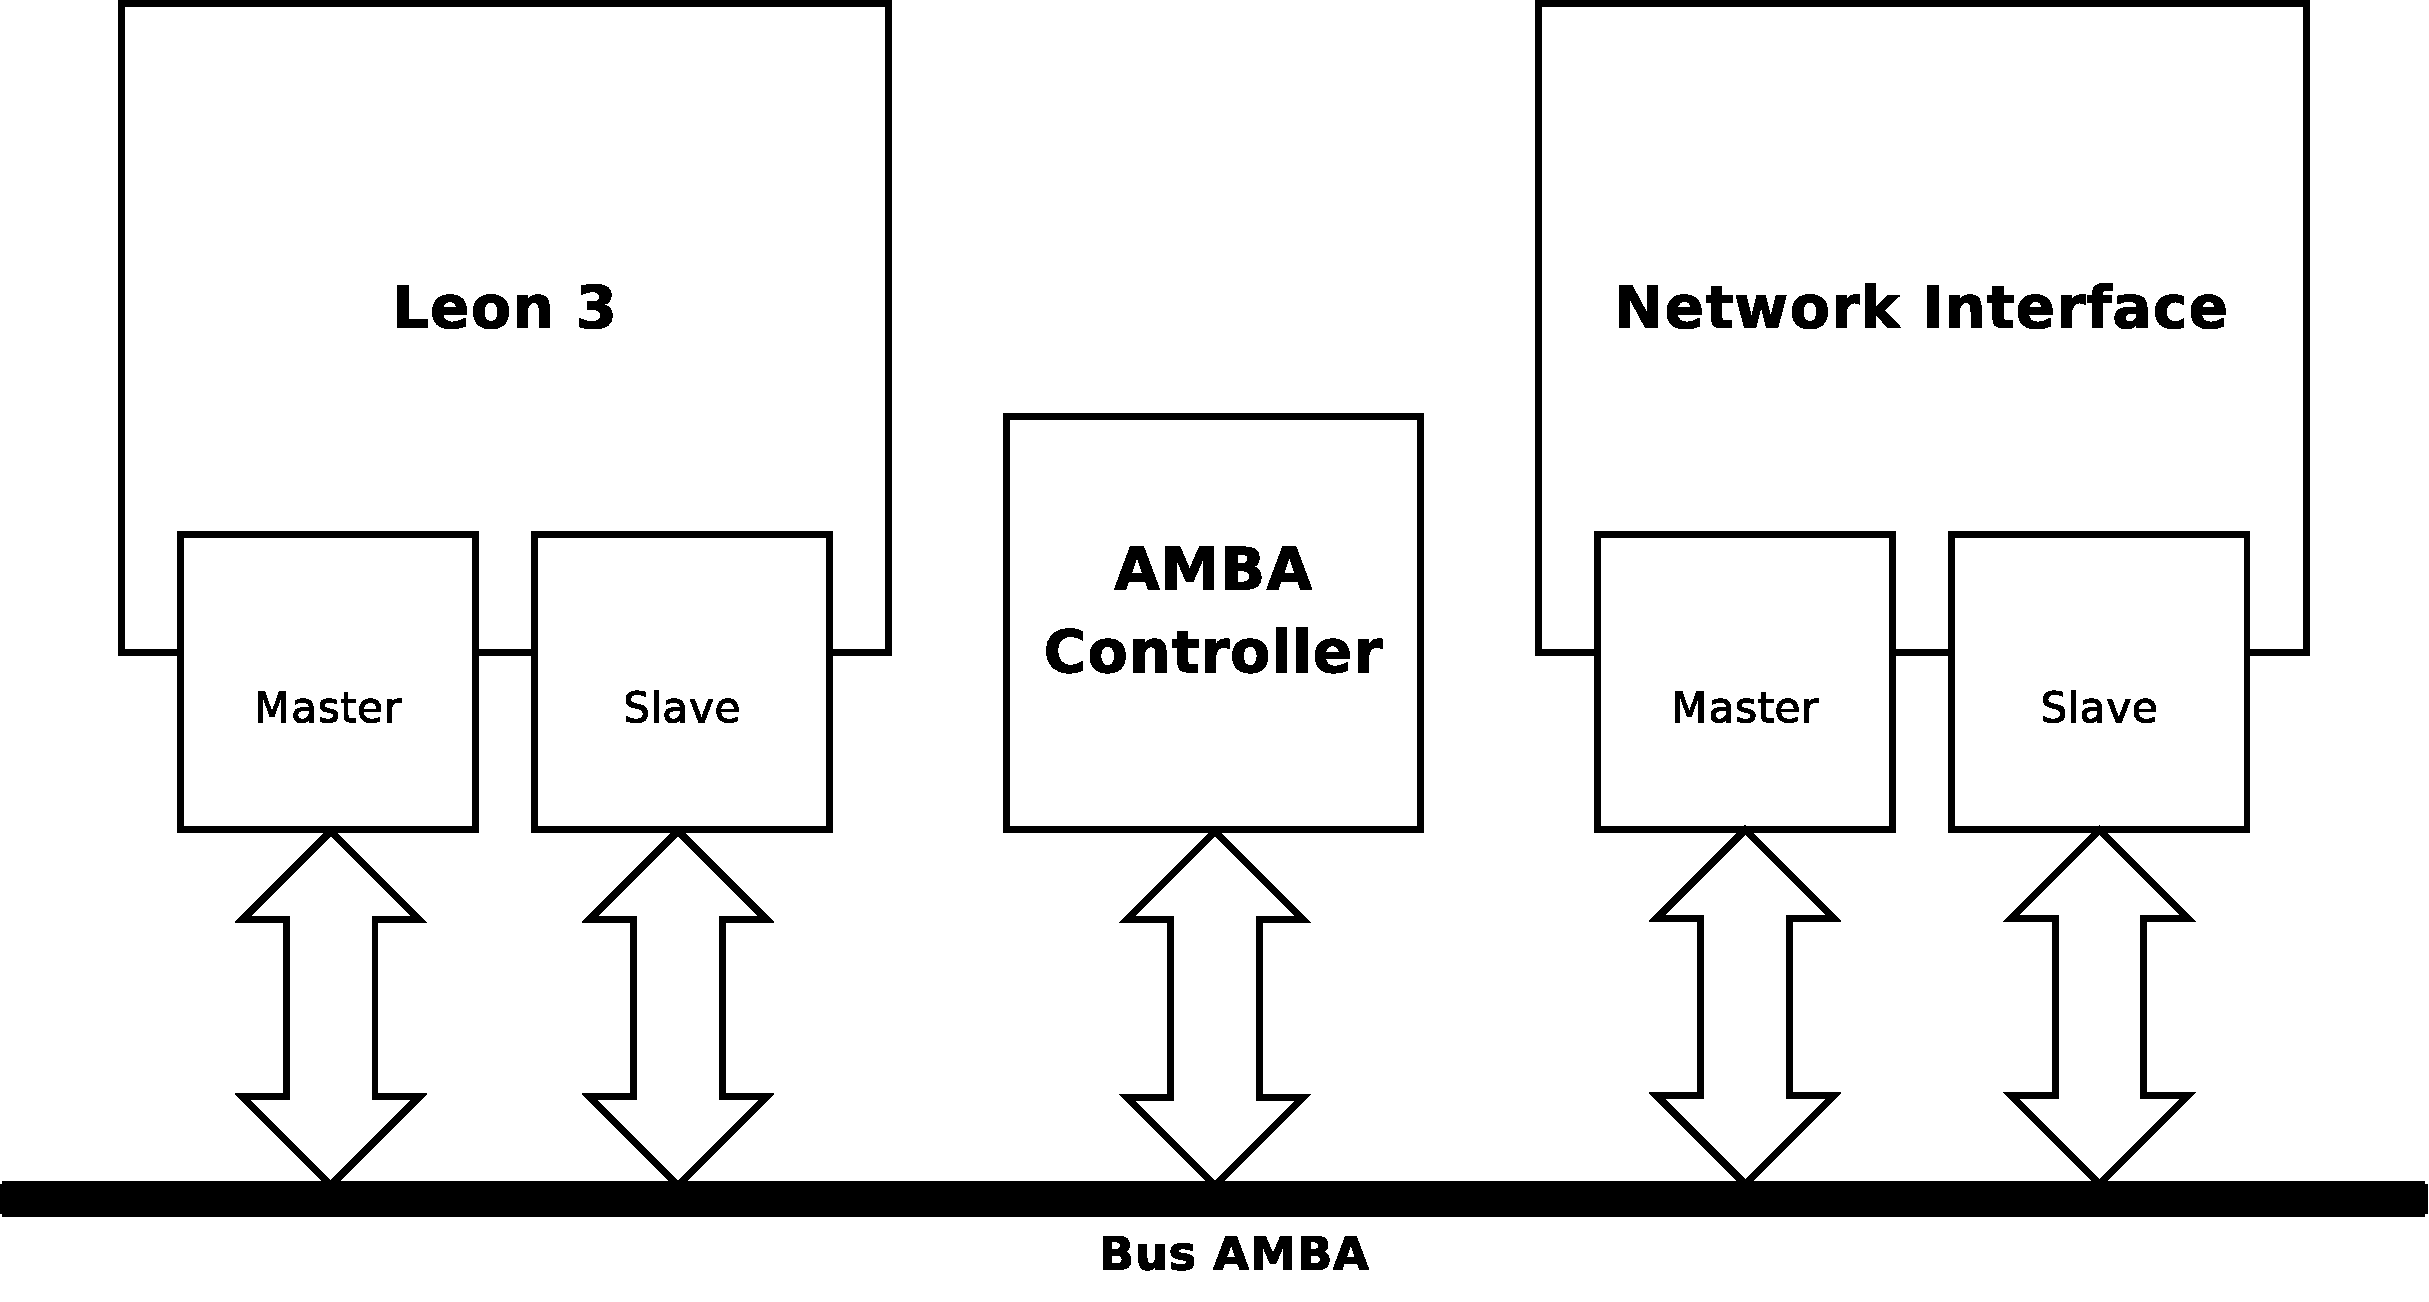
\includegraphics[width=0.9\textwidth]{fig/schem/bus_general}
\end{center}

Para evitar conflictos, las direcciones se mapearán en un rango distinto, aprovechando que el bus de direcciones es de 32 bits y sólo se aprovechan 16, se podran dividir en dos grupos: 0xXXXXYYYY, dónde XXXX será 0 para las direcciones de la red, y distinto de 0 para el resto. 

En el bus, el master por defecto será el procesador, pero la interface tendrá más prioridad.

\subsection*{Ejemplos de transferencias}

Aquí podemos ver unos ejemplos de transferencias. Primero tenemos una transferencia simple, de sólo un dato:

\begin{center}
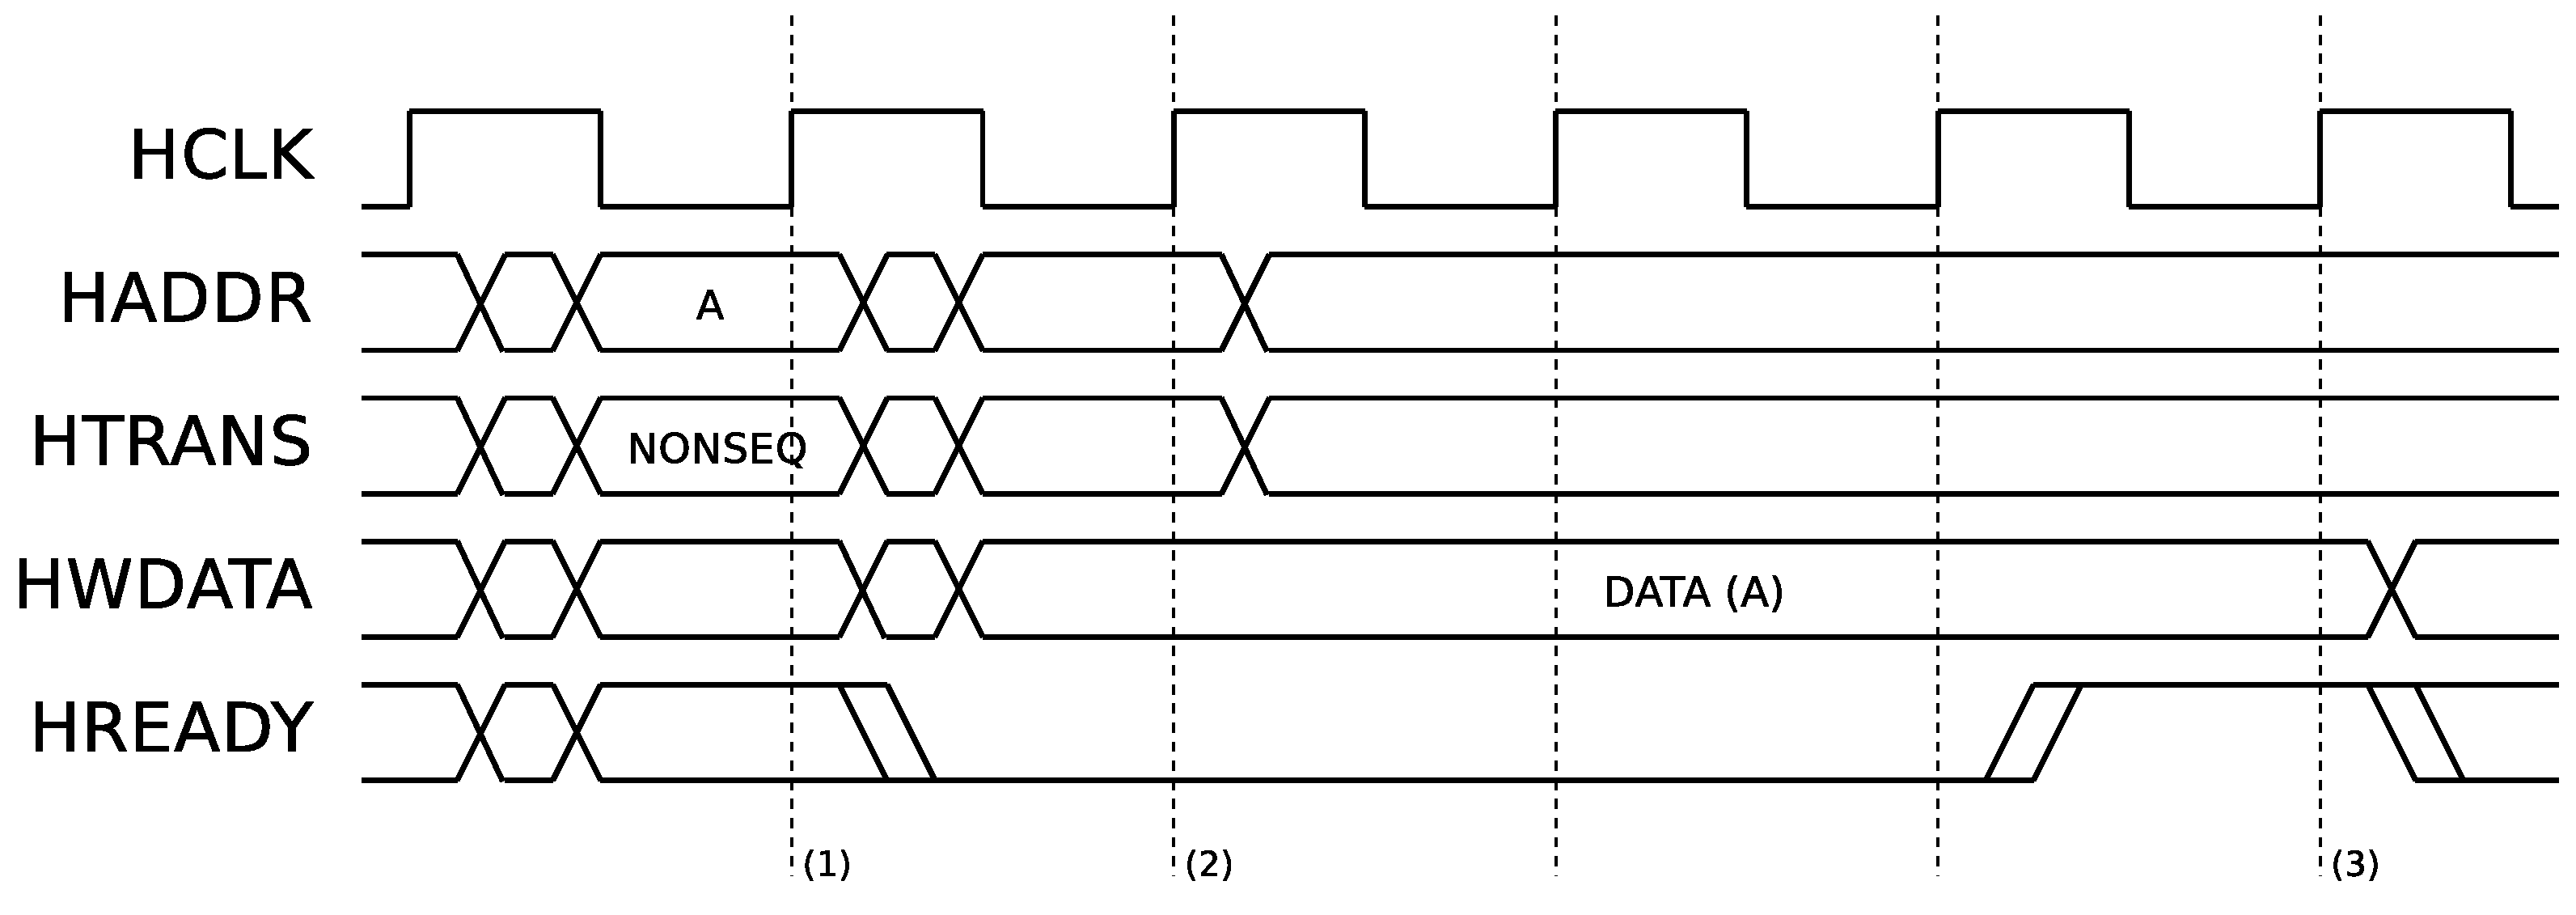
\includegraphics[width=0.9\textwidth]{fig/waves/trans_norm}
\end{center}

\begin{floatingfigure}[r]{0.3\textwidth}
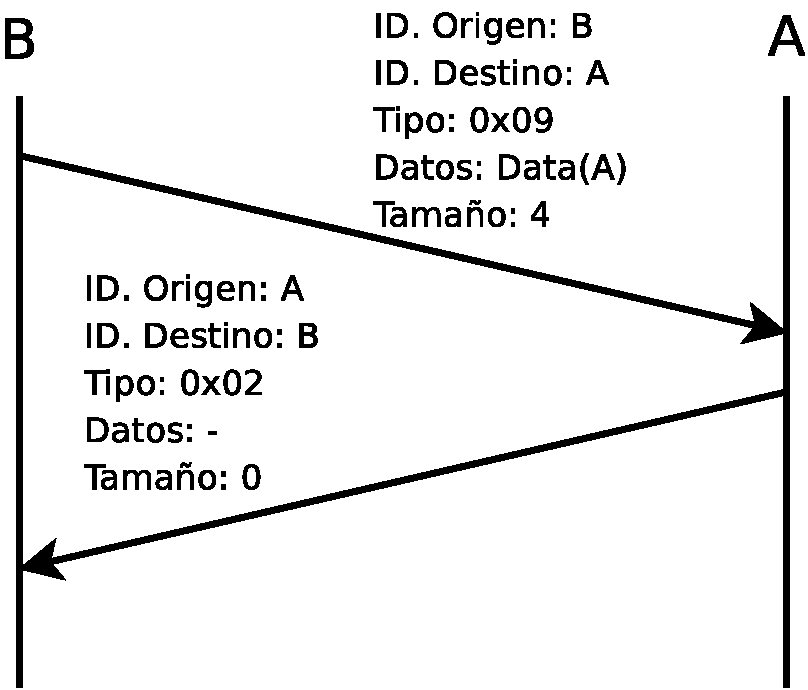
\includegraphics[width=0.3\textwidth]{fig/waves/net_norm}
\end{floatingfigure}

En (1), nos damos cuenta de que es el inicio de una conexión. Por lo tanto reseteamos los contadores de paquetes y nos preparamos para enviar el paquete de inicio de conexión.

En (2), ya tenemos los datos preparados, y los enviamos en un paquete con el tipo 0x09. Mientras no nos llega la confirmación, ponemos la señal \emph{HREADY} a 0, haciendo esperar el master.

Antes (3) nos ha llegado el paquete de confirmación de el otro nodo, por lo tanto, damos la transferencia por concluida y ponemos \emph{HREADY} a 1.

Por lo tanto, en esta transferencia se envían dos paquetes. El tipo del primer paquete enviado es 0x09, ya que es un paquete de escritura y de inicio de conexión, por lo tanto el campo de tipo tendrá activados los flags que corresponden.

\newpage

En la siguiente transferencia, tenemos una transferencia secuencial:

\begin{center}
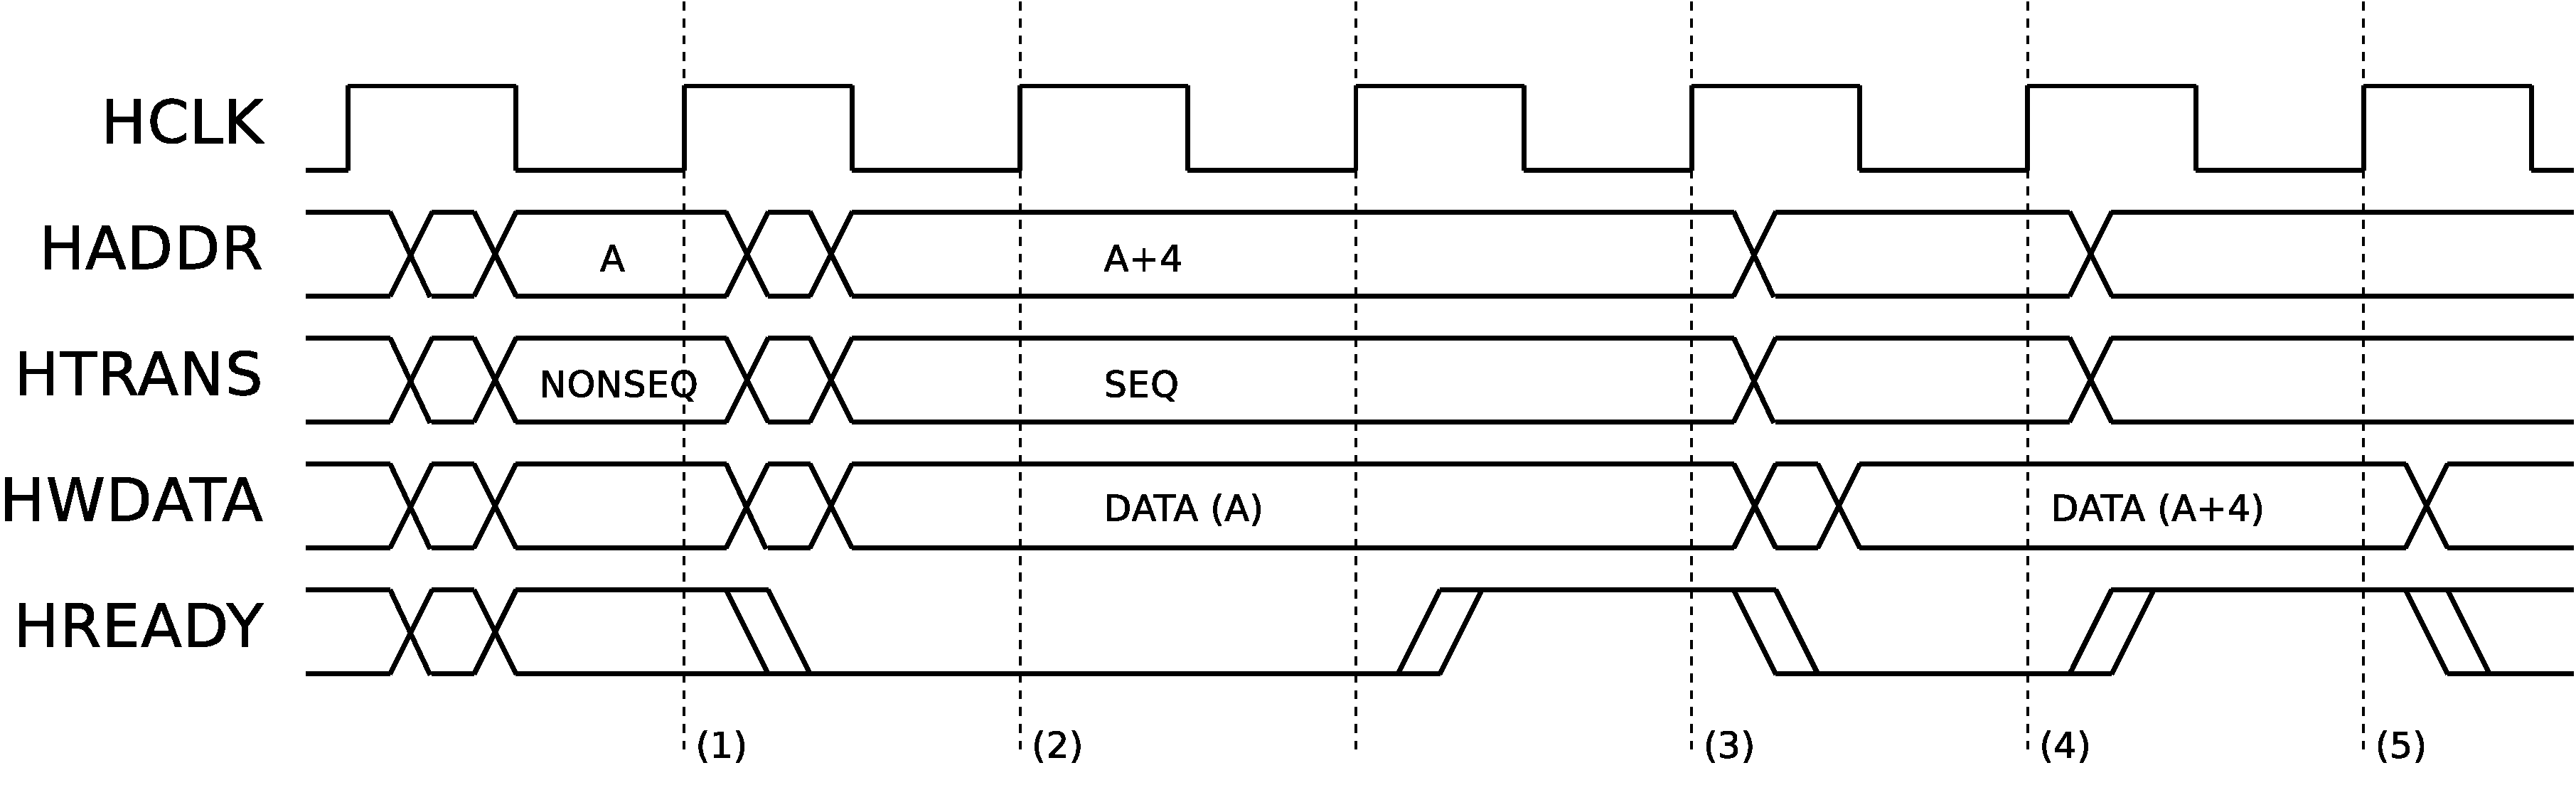
\includegraphics[width=0.9\textwidth]{fig/waves/trans_seq}
\end{center}

\begin{floatingfigure}[r]{0.3\textwidth}
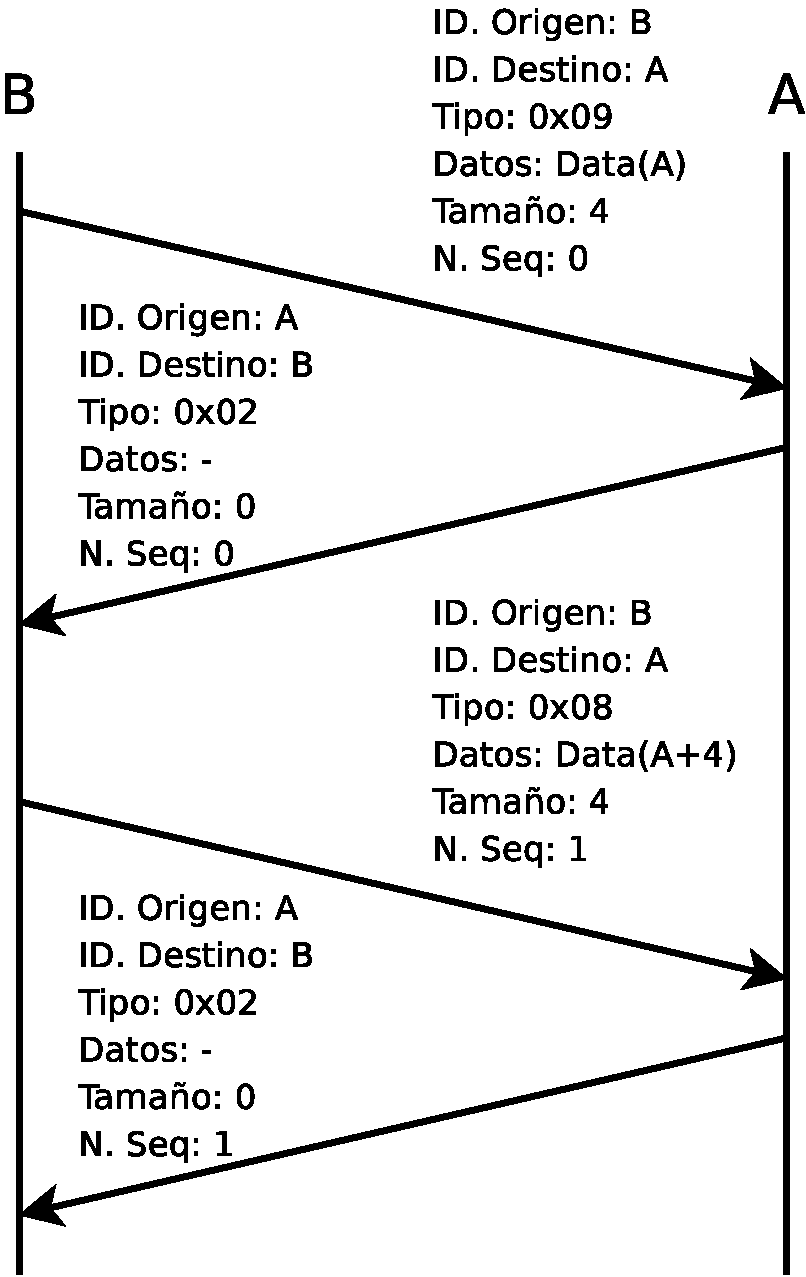
\includegraphics[width=0.3\textwidth]{fig/waves/net_seq}
\end{floatingfigure}

Cómo en la transferencia anterior, en (1) nos damos cuenta que es una nueva conexión, por lo tanto, el paquete que se envía en (2) es de tipo 0x09 (escritura + inicio de conexión).

En (3) hemos recibido la confirmación del primer paquete, y en (5) la del segundo que hemos enviado.

El paquete de datos que enviamos en (4), tiene el tipo 0x08, ya que sólo tiene activos el flag de transferencia de escritura.

Tenemos tres tipos de transferencias secuenciales (indicadas en el campo \emph{HBURST}):

\begin{itemize}
\item Una sola transferencia (SINGLE)
\item Ráfagas incrementales (INCR, INCR4, INCR8, INCR16)
\item Ráfagas cíclicas (WRAP4, WRAP8, WRAP16)
\end{itemize}

Para las ráfagas incrementales (y una sola transferencia) no hay ningún problema para deshacer el cambio que hacemos en la dirección, ya que sólo tendremos que sumar el tamaño de los paquetes a la dirección de destino.

En el caso de las transferencias cíclicas, hay un tipo de paquete para cada modo (WRAP4, WRAP8, WRAP16). Con este flag y el tamaño, el destino puede saber cuando hacer el \emph{wrapping} teniendoo en cuenta:

\begin{displaymath}
HADDR_{low} \\ = HADDR_{initial} - ( HADDR_{initial} mod (HSIZE * LEN_{burst})) 
\newline
HADDR_{high} \\ = HADDR_{low} + HSIZE * LEN_{burst}
\end{displaymath}

\newpage

\section*{Diagramas}

\subsection*{Entradas y salidas de la interfície}

\begin{figure}[h]
\centering
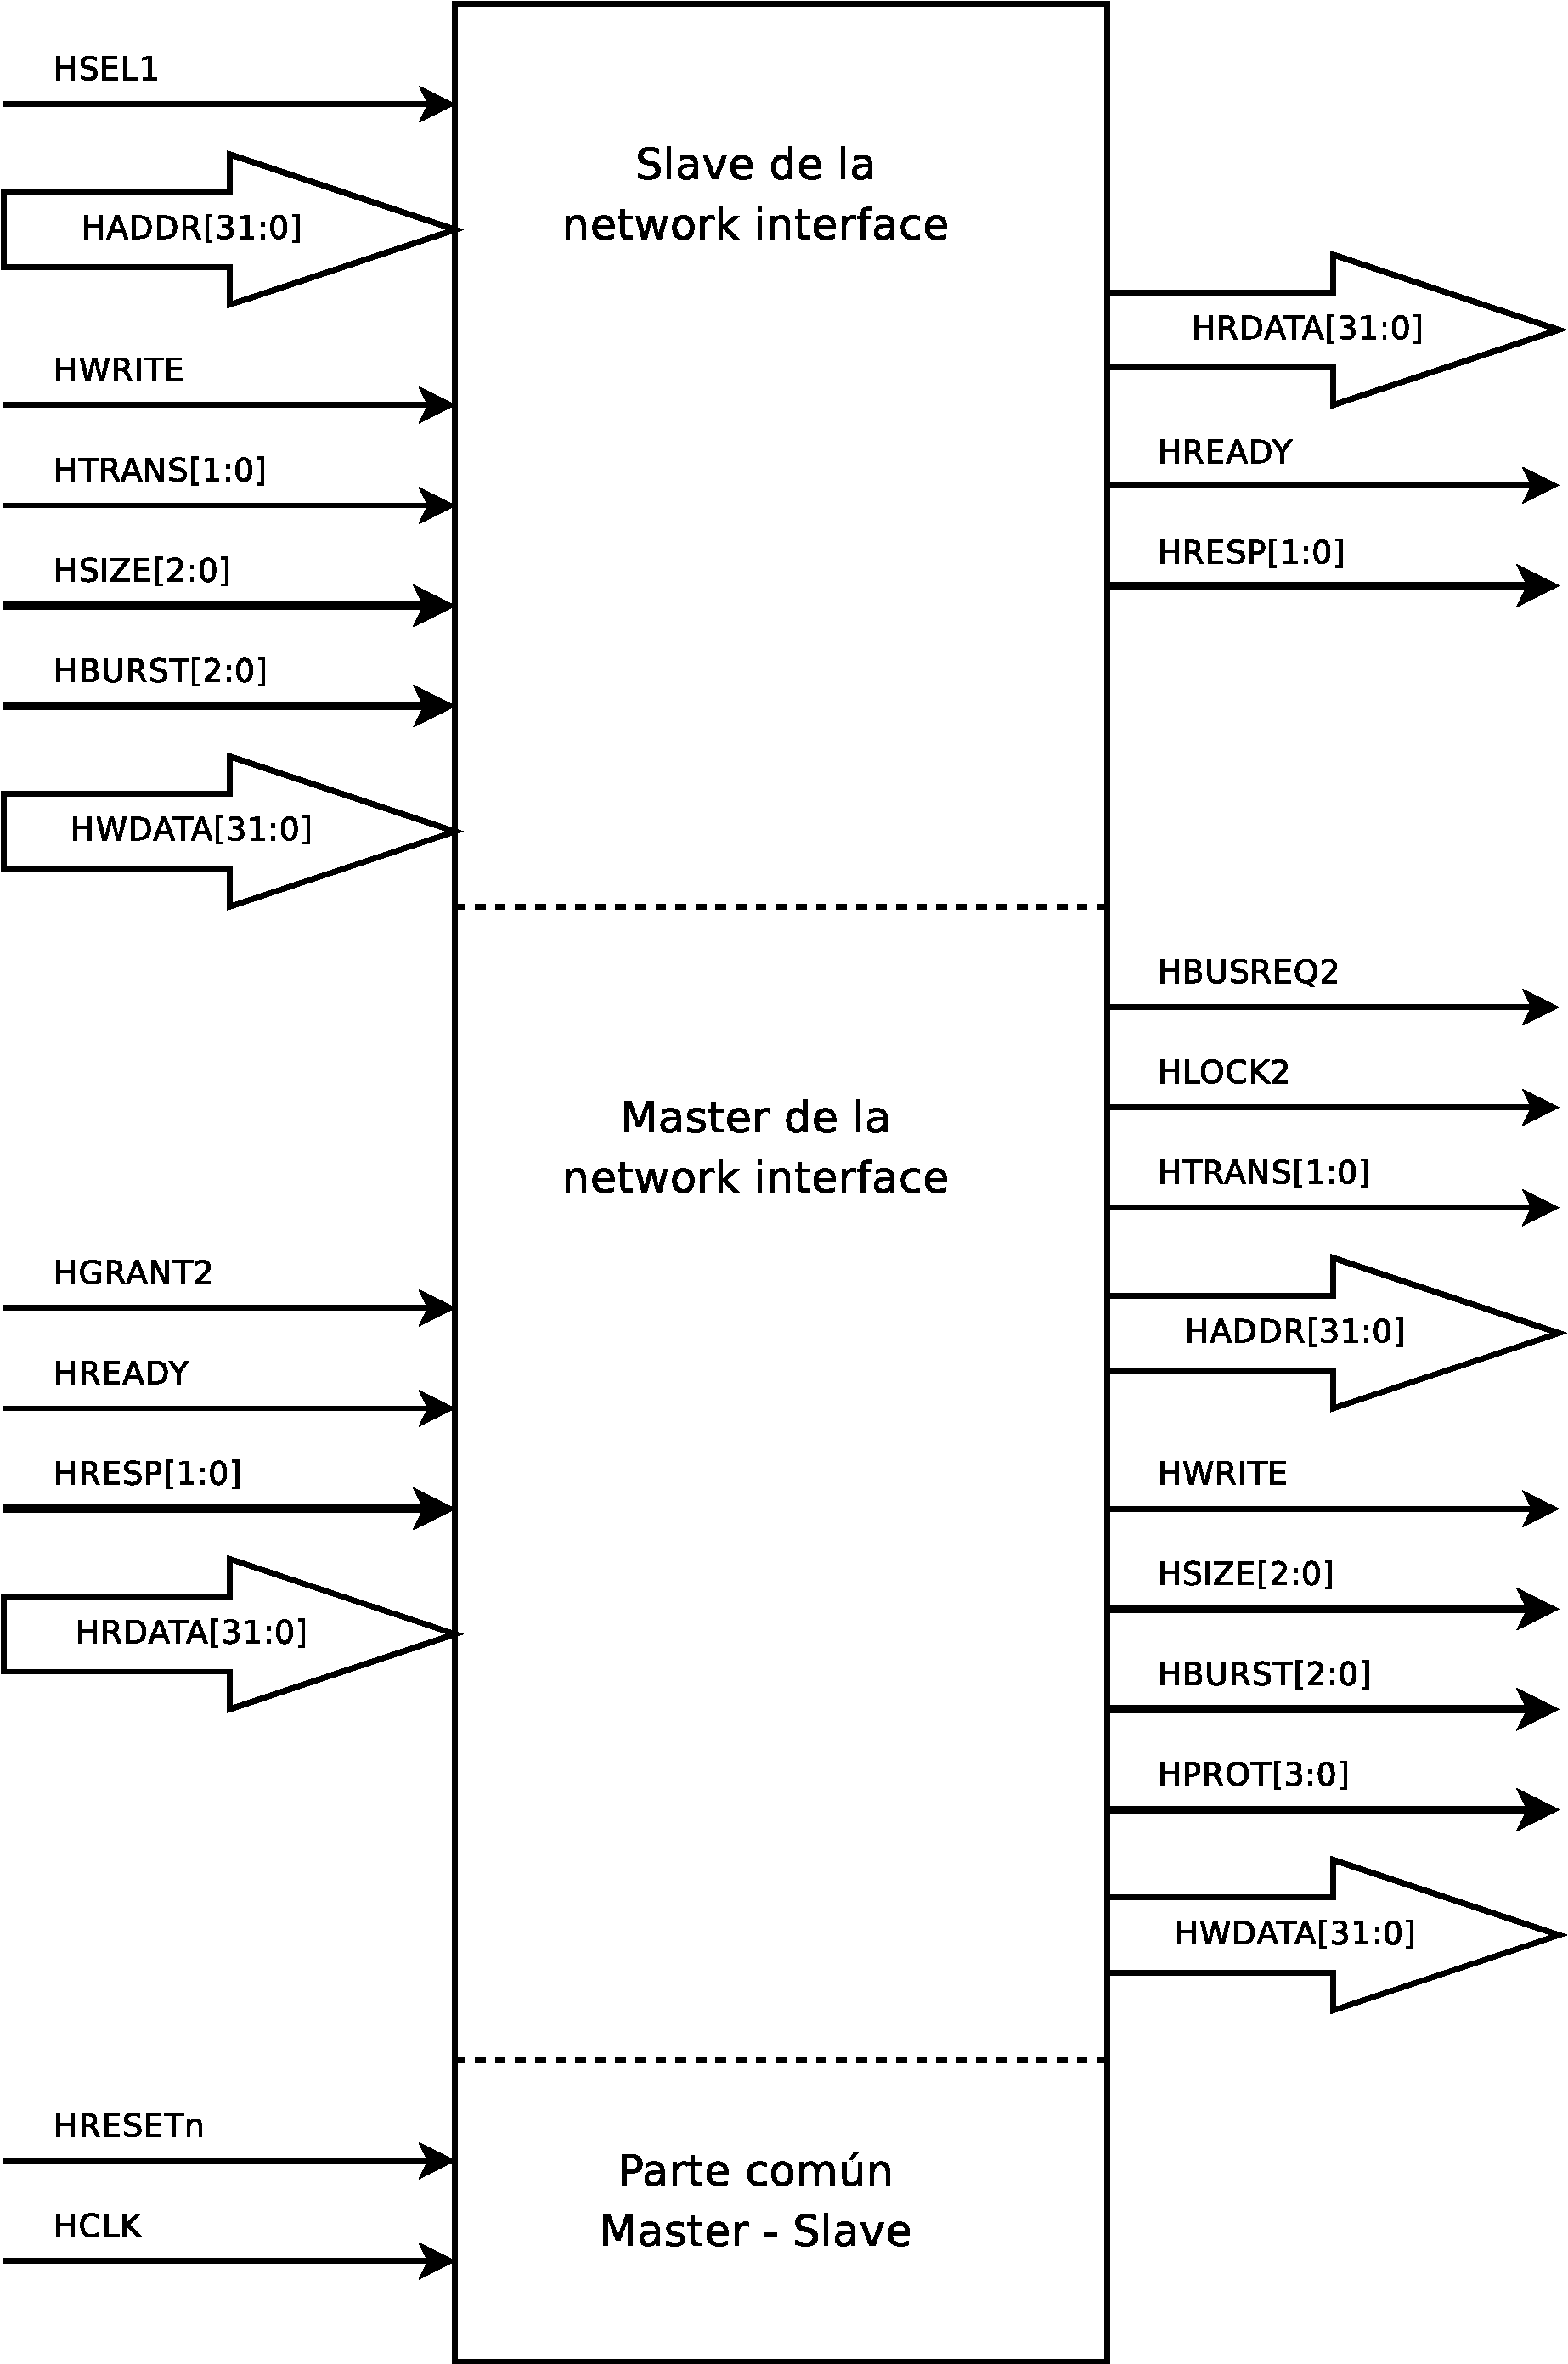
\includegraphics[width=0.7\textwidth]{fig/schem/top_ni}
\caption{Entradas y salidas por parte del procesador}
\end{figure}

\newpage

\begin{figure}[h]
\centering
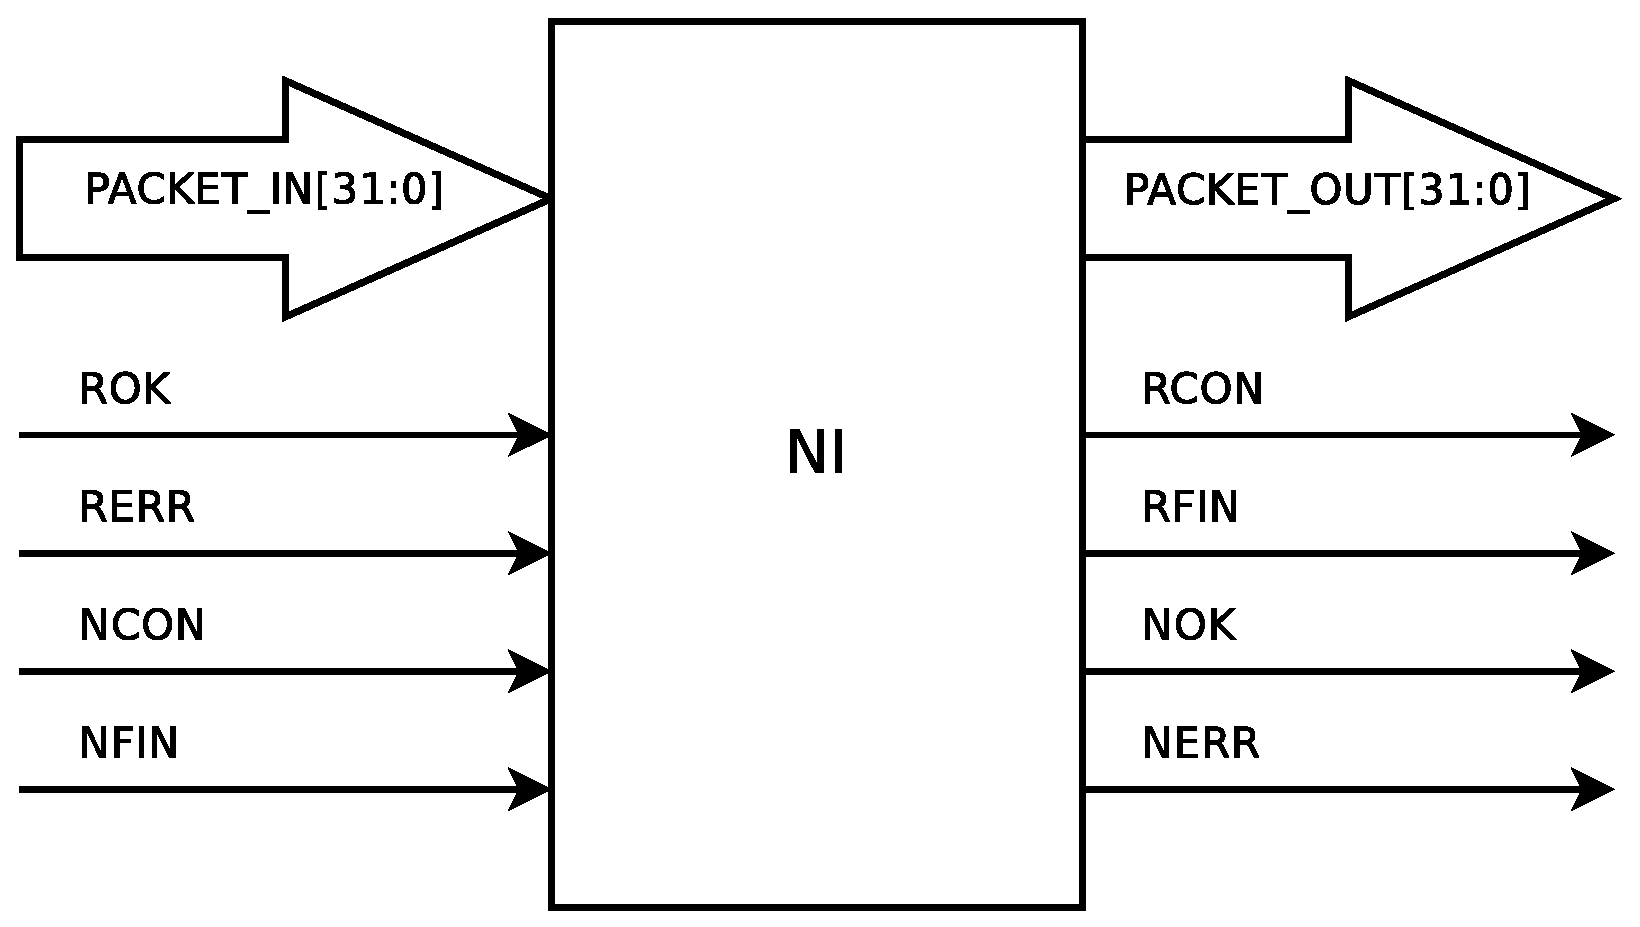
\includegraphics[width=0.7\textwidth]{fig/schem/top_ni_net}
\caption{Entradas y salidas por parte de la red}
\end{figure}

En la segunda figura, a parte de los buses que llevarán los paquetes, tenemos unas señales de \emph{handshake}:

\begin{description}
\item[RCON] se activa cuando la NI quiere empezar a enviar un paquete.
\item[RFIN] se activa cuando la NI ya ha acabado de enviar el paquete.
\item[ROK]  se activa cuando el router está preparado para recibir el paquete.
\item[RERR] se activa cuando ha habido algun error en el router. Se volverá a enviar el paquete.
\item[NCON] se activa cuando el router quiere empezar a enviar un paquete.
\item[NFIN] se activa cuando el router ya ha acabado de enviar el paquete.
\item[NOK]  se activa cuando la NI está preparada para recibir el paquete.
\item[NERR] se activa cuando ha habido algun error en la NI. Se volverá a enviar el paquete.
\end{description}

\newpage

\begin{landscape}
\subsection*{Circuitos}
\begin{figure}[h]
\centering
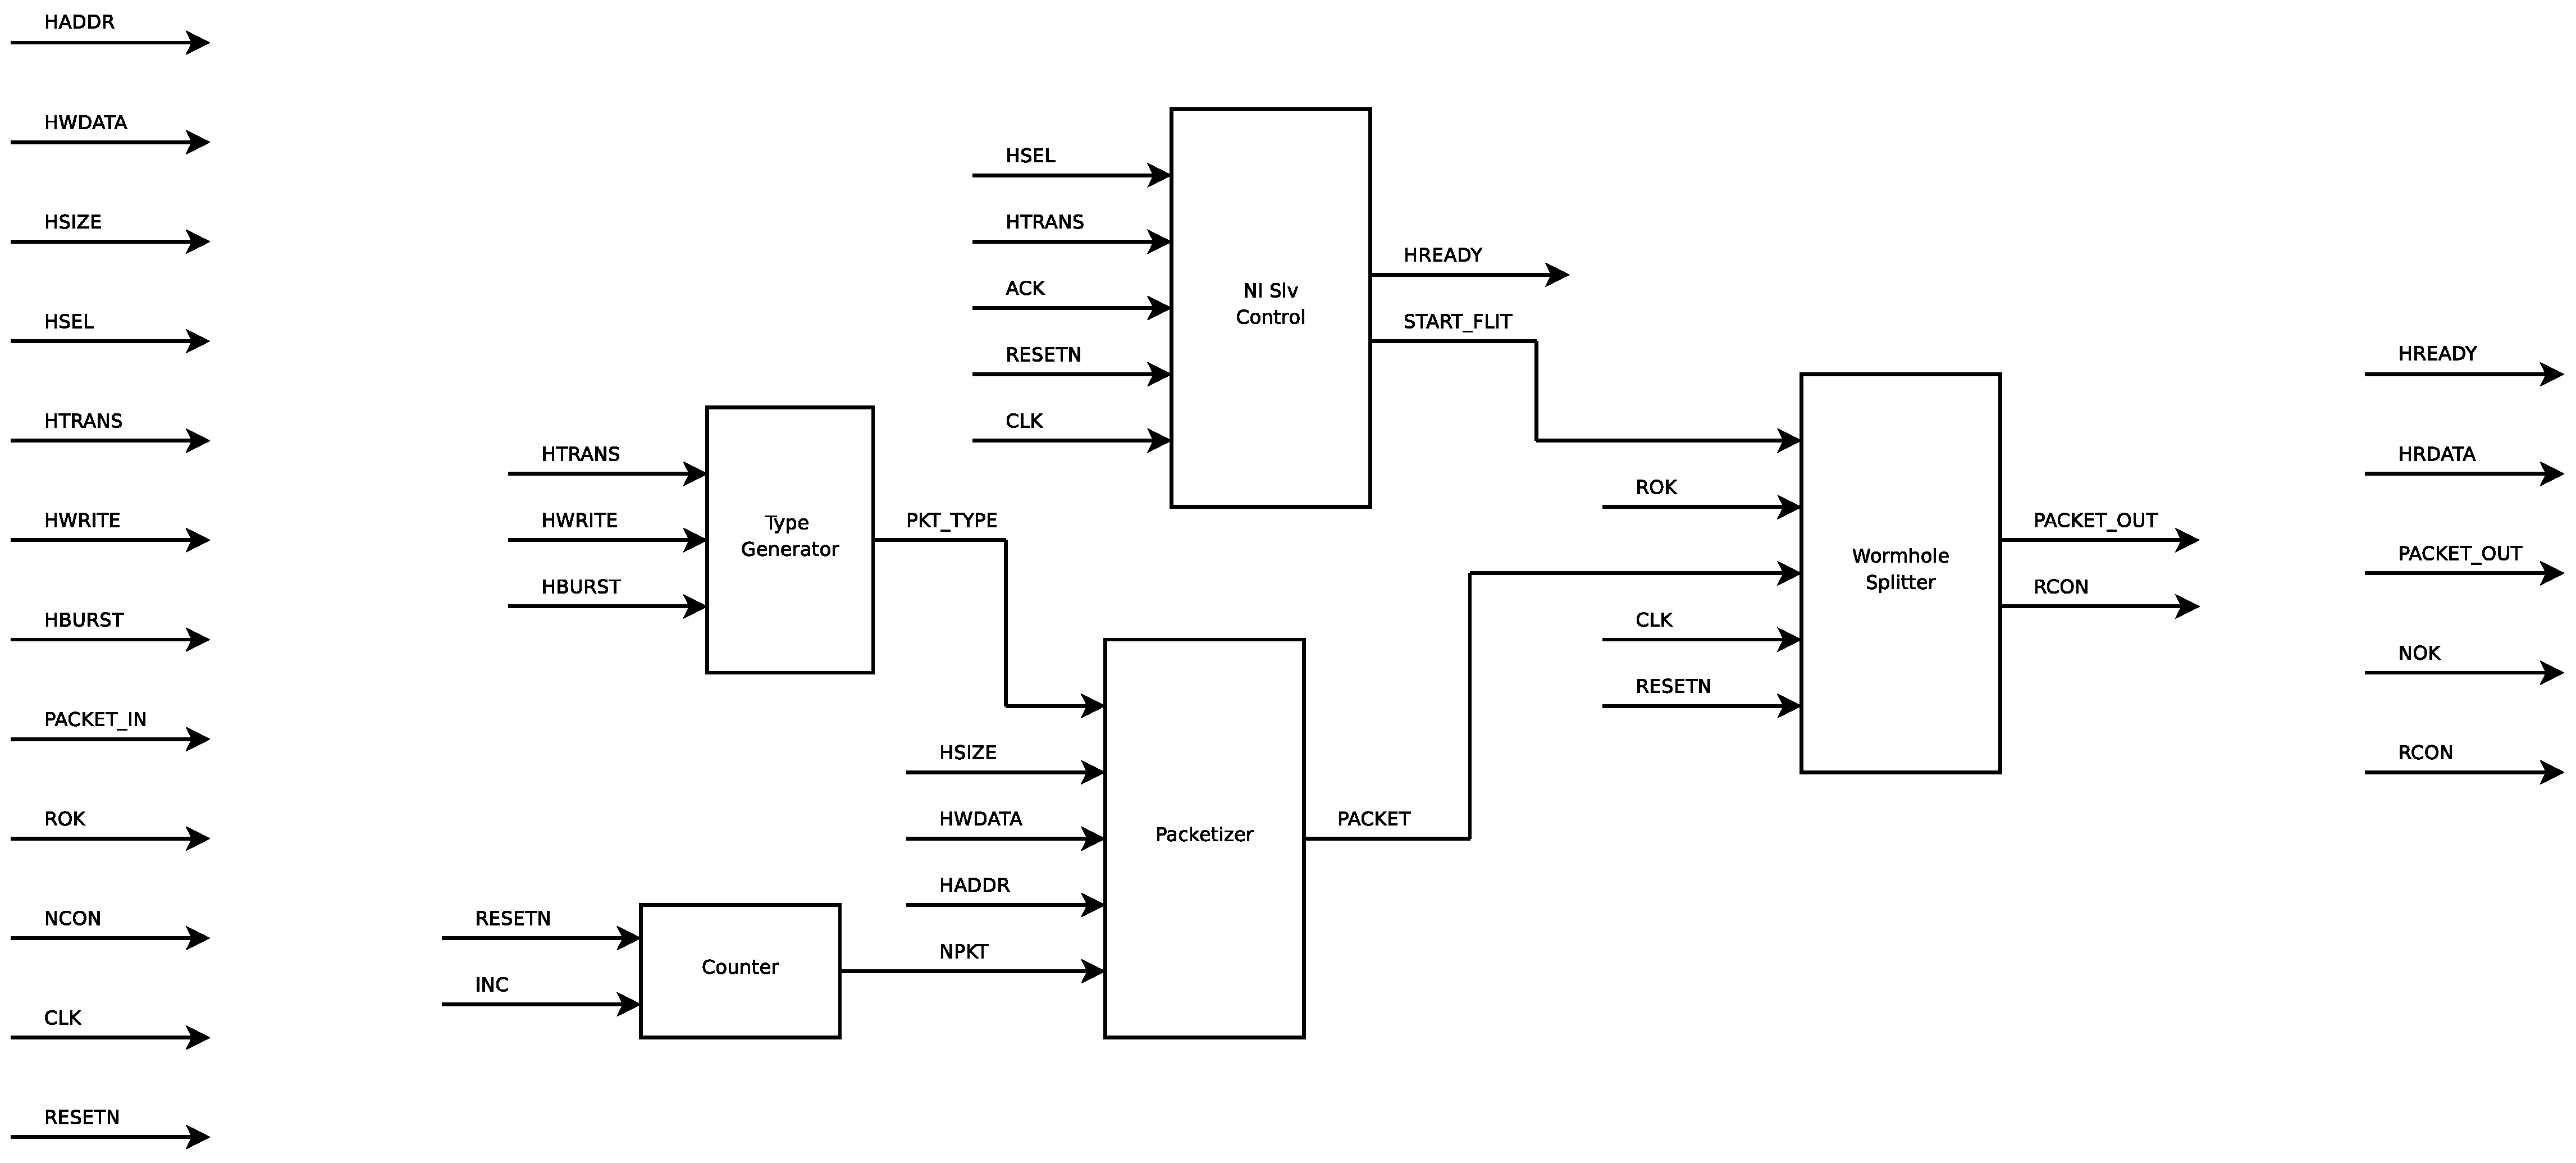
\includegraphics[width=1.5\textwidth]{fig/schem/NI}
\caption{Esquema del top de la NI}
\end{figure}
\end{landscape}

\end{document}
